\documentclass[aspectratio=169,11pt]{beamer}
\usepackage{tikz}
\usetikzlibrary{arrows.meta,positioning,fit,calc,matrix}
\usepackage{booktabs}
\graphicspath{{../report/generated/}}

% Palette shared with the report figures.
\definecolor{ink}{HTML}{1F2328}
\definecolor{muted}{HTML}{5E6168}
\definecolor{ordblue}{HTML}{2A78D6}
\definecolor{deporange}{HTML}{EB6834}
\definecolor{lenaqua}{HTML}{1BAF7A}
\definecolor{paper}{HTML}{FCFCFB}
\definecolor{rule}{HTML}{E4E3DF}

\setbeamercolor{background canvas}{bg=paper}
\setbeamercolor{normal text}{fg=ink}
\setbeamercolor{frametitle}{fg=ink}
\setbeamercolor{structure}{fg=deporange}
\setbeamercolor{itemize item}{fg=deporange}
\setbeamercolor{block title}{fg=ink,bg=rule}
\setbeamerfont{frametitle}{size=\Large,series=\bfseries}
\setbeamertemplate{navigation symbols}{}
\setbeamertemplate{itemize item}{\small$\blacktriangleright$}
\setbeamertemplate{footline}{%
  \hspace{1em}\textcolor{muted}{\scriptsize\insertshortauthor\hfill\insertframenumber/\inserttotalframenumber}\hspace{1em}\vspace{.6em}}

\newcommand{\speaker}[1]{\par\vspace{-1.2em}\hfill\textcolor{muted}{\scriptsize Speaker: #1}\par\vspace{.2em}}
\newcommand{\pos}[1]{\textcolor{deporange}{\textbf{#1}}}

\title{Dependency-Preserving Evidence Packing\\for Numerical Question Answering}
\author[Pushpendra Singh \& Badri Bishal Das]{Pushpendra Singh \and Badri Bishal Das}
\date{Big Data course project}

\tikzset{
  box/.style={draw=muted,rounded corners=3pt,fill=white,align=center,font=\footnotesize,minimum height=8mm,inner xsep=4pt},
  hot/.style={box,draw=deporange,line width=1pt},
  arrow/.style={-{Stealth[length=2.2mm]},muted,thick},
  cell/.style={draw=rule,minimum height=5.5mm,font=\scriptsize,inner xsep=3pt},
}

\begin{document}

% 1 ---------------------------------------------------------------
\begin{frame}[plain]
\vfill
{\usebeamerfont{title}\Large\bfseries \inserttitle\par}
\vspace{1em}
{\large Pushpendra Singh \quad Badri Bishal Das\par}
\vspace{.4em}
{\textcolor{muted}{Big Data course project \textbullet{} FinQA, ConvFinQA, TAT-QA, HybridQA, TAT-HQA, MultiHiertt}\par}
\vfill
\note{Speaker A opens. One sentence: when a model can only read part of a document,
does keeping each number's labels with it help? Introduce both speakers and the split.}
\end{frame}

% 2 ---------------------------------------------------------------
\begin{frame}{A number means nothing without its labels}
\speaker{A}
\begin{columns}[T]
\column{.56\textwidth}
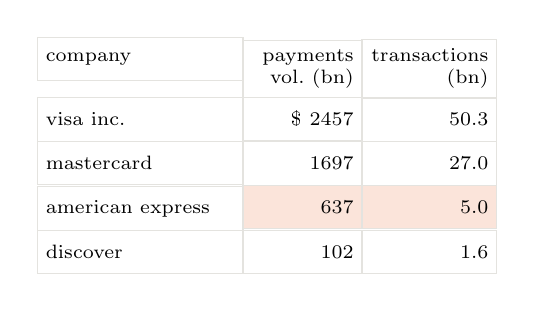
\begin{tikzpicture}[node distance=0pt]
\matrix (t) [matrix of nodes, ampersand replacement=\&, nodes={cell}, column sep=-\pgflinewidth, row sep=-\pgflinewidth,
  column 1/.style={nodes={text width=24mm}}, column 2/.style={nodes={text width=13mm,align=right}},
  column 3/.style={nodes={text width=15mm,align=right}}]{
  company \& payments vol.\ (bn) \& transactions (bn)\\
  visa inc. \& \$ 2457 \& 50.3\\
  mastercard \& 1697 \& 27.0\\
  american express \& |[fill=deporange!18]| 637 \& |[fill=deporange!18]| 5.0\\
  discover \& 102 \& 1.6\\
};
\end{tikzpicture}
\vspace{.6em}

{\footnotesize\textcolor{muted}{Real FinQA development example. Gold program: \texttt{divide(637, const\_5)} $=127.4$}}
\column{.42\textwidth}
\textit{``What is the average payment volume per transaction for American Express?''}
\vspace{.8em}
\begin{itemize}\itemsep4pt
\item The answer needs \pos{two cells} plus the \pos{row label} and \pos{two column headers}.
\item Given ``637'' and ``5.0'' alone, the model cannot tell which is which.
\item With a small reading budget, labels compete with facts for space.
\end{itemize}
\end{columns}
\note{Point at the highlighted cells. The question is what to keep when you cannot
keep everything: the facts, or the facts together with what makes them readable.}
\end{frame}

% 3 ---------------------------------------------------------------
\begin{frame}{Research question and data}
\speaker{A}
\begin{block}{Question}
With the \pos{same model} and the \pos{same evidence budget}, does keeping each fact's
headers, units, hierarchy and links with it improve answers over ordinary packing?
\end{block}
\vspace{.4em}
\begin{columns}[T]
\column{.5\textwidth}
\footnotesize
\begin{tabular}{@{}llr@{}}
\toprule
& Dataset & Dev questions\\\midrule
Assigned & FinQA & 883\\
& ConvFinQA & 1,490 turns\\
& TAT-QA & 1,668\\
& HybridQA & 3,466\\
Added & TAT-HQA & 824\\
& MultiHiertt & 1,044\\\bottomrule
\end{tabular}
\column{.46\textwidth}
\begin{itemize}\itemsep3pt\footnotesize
\item One shared pipeline; only readers and scorers differ per dataset.
\item Official evaluators, run unchanged at pinned versions.
\item Related datasets share documents, so results are \pos{never pooled}.
\item HybridQA is general knowledge: a transfer test, not finance.
\end{itemize}
\end{columns}
\note{Stress the controlled comparison: model, prompt and budget fixed; only the packing
method changes. Feeding gold answers through each official scorer gives 100\% on five datasets; MultiHiertt gives 90.5\% because its span path drops minus signs.}
\end{frame}

% 4 ---------------------------------------------------------------
\begin{frame}{One pipeline for six datasets}
\speaker{A}
\centering
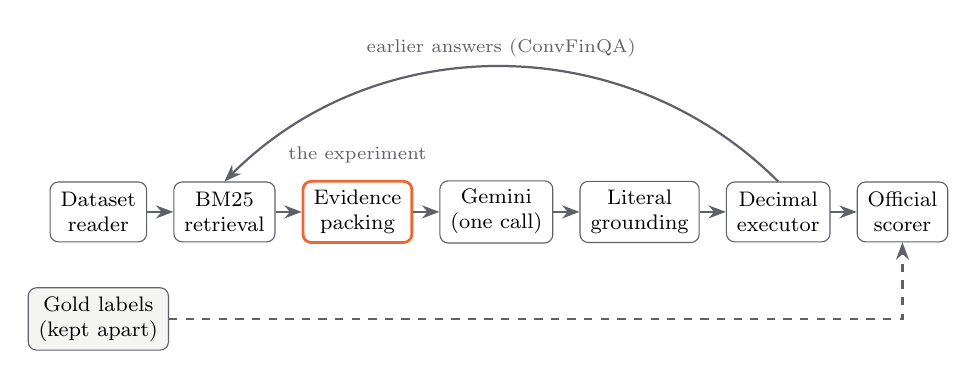
\begin{tikzpicture}[node distance=3.5mm,scale=.95,transform shape]
\node[box] (read) {Dataset\\reader};
\node[box,right=of read] (ret) {BM25\\retrieval};
\node[hot,right=of ret] (pack) {Evidence\\packing};
\node[box,right=of pack] (llm) {Gemini\\(one call)};
\node[box,right=of llm] (ground) {Literal\\grounding};
\node[box,right=of ground] (exec) {Decimal\\executor};
\node[box,right=of exec] (score) {Official\\scorer};
\foreach \a/\b in {read/ret,ret/pack,pack/llm,llm/ground,ground/exec,exec/score}\draw[arrow] (\a)--(\b);
\node[box,below=6mm of read,fill=rule!40] (labels) {Gold labels\\(kept apart)};
\draw[arrow,dashed] (labels.east) -| (score.south);
\node[font=\scriptsize,muted,above=1mm of pack] {the experiment};
\draw[arrow] (exec.north) to[out=135,in=45] node[above,font=\scriptsize,muted]{earlier answers (ConvFinQA)} (ret.north);
\end{tikzpicture}
\vspace{.3em}
\begin{columns}[T]
\column{.48\textwidth}
\footnotesize
\begin{itemize}\itemsep3pt
\item Each fact stores its text and the IDs of the facts needed to read it.
\item Labels never reach the prompt: 0 of 443 inspected prompts contained one.
\end{itemize}
\column{.48\textwidth}
\footnotesize
\begin{itemize}\itemsep3pt
\item Every raw response is saved, so runs resume and re-score without new calls.
\item Spark builds the deduplicated fact store, checked against Python.
\end{itemize}
\end{columns}
\note{Walk left to right once. Only the orange box changes between methods.}
\end{frame}

% 5 ---------------------------------------------------------------
\begin{frame}{Three ways to pack the same budget}
\speaker{A}
\begin{columns}[T]
\column{.33\textwidth}
\textcolor{ordblue}{\textbf{Ordinary (O)}}\par\vspace{.3em}
{\scriptsize\ttfamily amex | payments | 637\\amex | txns | 5.0\par}
\vspace{.3em}{\footnotesize Labels repeated inline per cell. A fair baseline, not a weakened one.}
\column{.33\textwidth}
\textcolor{deporange}{\textbf{Dependency (D)}}\par\vspace{.3em}
{\scriptsize\ttfamily company | payments | txns\\amex | 637 | 5.0\par}
\vspace{.3em}{\footnotesize Recursive closure of headers, units, hierarchy and links, stored once.}
\column{.33\textwidth}
\textcolor{lenaqua}{\textbf{Length-matched (L)}}\par\vspace{.3em}
{\scriptsize\ttfamily 637 \ 5.0 \ 102 \ 1.6\par}
\vspace{.3em}{\footnotesize Neighbouring facts up to D's length. Tests whether \emph{more text} is enough.}
\end{columns}
\vspace{1em}
\begin{block}{Literal grounding: the model copies values, code finds them}
\footnotesize The model writes \texttt{divide("637", "5.0")}. We locate each value in the packed
evidence or the question; a value found nowhere rejects the answer. The earlier design asked for
character offsets and reached \pos{2 of 883} FinQA questions. That run also used a different model,
so we do not credit the format alone.
\end{block}
\note{This is the key mechanism slide. Hand over to speaker B after it.}
\end{frame}

% 6 ---------------------------------------------------------------
\begin{frame}{A fair experiment on a free-tier budget}
\speaker{B}
\begin{columns}[T]
\column{.5\textwidth}
\textbf{Budget must actually bind}
\begin{itemize}\itemsep3pt\footnotesize
\item At 4,000 tokens, four datasets were not truncated in a 40-question sample: methods would differ only in layout.
\item Caps chosen from document sizes, without labels: 400--1,500 tokens.
\end{itemize}
\vspace{.5em}
\textbf{Three measurements}
\begin{itemize}\itemsep3pt\footnotesize
\item \pos{Coverage}: does gold evidence survive packing? All 9,268 questions, no model.
\item \pos{Block A}: O vs D vs L answers, \texttt{gemini-3.5-flash-lite}.
\item \pos{Block B}: executor vs direct answering, \texttt{gemini-3.1-flash-lite}.
\end{itemize}
\column{.46\textwidth}
\textbf{Rules}
\begin{itemize}\itemsep3pt\footnotesize
\item One model per comparison; models are never compared with each other.
\item Samples fixed by seed before any call; conversations kept whole.
\item Failures stay in the denominator as zero.
\item Paired bootstrap over whole documents, 2,000 resamples.
\item 500 requests per day per model: runs stop and resume from saved answers.
\end{itemize}
\end{columns}
\note{The cap choice is the most important design fix: an unbinding budget makes the
comparison meaningless.}
\end{frame}

% 7 ---------------------------------------------------------------
\begin{frame}{Result 1: dependency packing keeps more gold evidence}
\speaker{B}
\centering
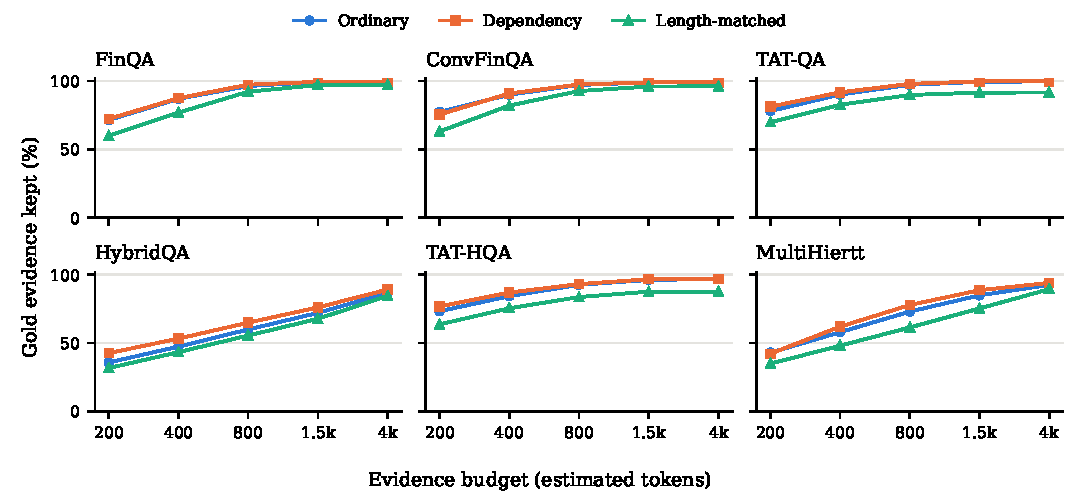
\includegraphics[width=.74\textwidth]{coverage_wide.pdf}\par
\vspace{.2em}
{\footnotesize Exact counts over every scorable development question. Questions kept only by D vs only by O at the chosen cap:
HybridQA \pos{146 vs 7}, MultiHiertt \pos{42 vs 3}, TAT-QA 41 vs 15, TAT-HQA 33 vs 12, FinQA 9 vs 1, ConvFinQA 6 vs 1.
At 200 tokens the closure overhead costs coverage on ConvFinQA and MultiHiertt.}
\note{Two observations. D is above O on all six datasets at the chosen caps, most where documents are
large. The gap closes as budgets grow, which is exactly what the hypothesis predicts.
L is lowest: more nearby text is not the same as the right labels.
At 200 tokens the closure overhead costs coverage on ConvFinQA and MultiHiertt: a measured limit.}
\end{frame}

% 8 ---------------------------------------------------------------
\begin{frame}{Result 2: effect on answers}
\speaker{B}
\begin{columns}[T]
\column{.5\textwidth}
\textbf{Block A: packing (\%)}\par\vspace{.3em}
\scriptsize\setlength{\tabcolsep}{2.5pt}
\resizebox{\linewidth}{!}{\begin{tabular}{lrrrrrl}
Dataset & $n$ & O & D & L & D$-$O & 95\% CI\\\hline\noalign{\vskip 2pt}
FinQA & 50 & 62.0 & 64.0 & 66.0 & +2.0 & [+0.0, +6.2]\\
ConvFinQA & 45 & 73.3 & 73.3 & 68.9 & +0.0 & [$-$6.0, +6.4]\\
TAT-QA & 50 & 60.2 & 71.5 & 69.4 & +11.3 & [+4.1, +19.9]\\
HybridQA & 50 & 54.9 & 60.1 & 49.8 & +5.3 & [$-$2.4, +13.0]\\
TAT-HQA & 50 & 56.7 & 60.7 & 52.7 & +4.0 & [$-$6.4, +14.5]\\
MultiHiertt & 50 & 47.0 & 56.8 & 41.0 & +9.8 & [+0.0, +20.0]\\
\end{tabular}
}
\column{.48\textwidth}
\textbf{Block B: executor vs direct (\%)}\par\vspace{.3em}
\scriptsize\setlength{\tabcolsep}{2.5pt}
\resizebox{\linewidth}{!}{\begin{tabular}{lrrrrl}
Dataset & $n$ & Executor & Direct & Diff. & 95\% CI\\\hline\noalign{\vskip 2pt}
FinQA & 40 & 62.5 & 67.5 & $-$5.0 & [$-$17.5, +7.0]\\
ConvFinQA & 36 & 75.0 & 75.0 & +0.0 & [$-$8.6, +7.3]\\
TAT-QA & 40 & 65.2 & 58.7 & +6.5 & [$-$7.6, +20.7]\\
HybridQA & 40 & 50.2 & 66.6 & $-$16.4 & [$-$30.6, $-$2.0]\\
TAT-HQA & 40 & 60.0 & 56.7 & +3.3 & [$-$12.0, +19.3]\\
MultiHiertt & 40 & 63.7 & 41.7 & +22.1 & [+2.5, +40.0]\\
\end{tabular}
}
\end{columns}
\vspace{.6em}
\footnotesize
\begin{itemize}\itemsep2pt
\item Packing: D $\geq$ O on all six datasets; the interval excludes zero only on \pos{TAT-QA (+11.3)}.
\item Intervals are wide at these sample sizes; six comparisons per block are uncorrected.
\item Only robust Block B gap: \pos{direct answering wins on HybridQA}, which has short text answers and no arithmetic.
\item MultiHiertt's Block B row is official F1; under one scoring rule for both sides the gap is +6.2 (next slide).
\end{itemize}
\note{Read the D minus O column and its intervals. Do not over-claim: say what the intervals allow.}
\end{frame}

% 9 ---------------------------------------------------------------
\begin{frame}{What failed, and what we learned}
\speaker{B}
\begin{columns}[T]
\column{.5\textwidth}
\textbf{A result we withdrew}
\begin{itemize}\itemsep3pt\footnotesize
\item MultiHiertt first showed the executor \pos{+22.1} points ahead.
\item Direct answers wrote $-29.92$ for a gold $-0.2992$; the official span path marks that wrong.
\item Same scoring rule for both sides: \pos{+6.2}, interval [$-6.2$, $+20.0$]. No claim.
\end{itemize}
\vspace{.4em}
\textbf{Where answers still go wrong}
\begin{itemize}\itemsep3pt\footnotesize
\item Numbers: wrong values, reversed percentage-change direction.
\item Text: over-long or wrong spans (HybridQA, TAT-QA).
\item Validation failures are now rare.
\end{itemize}
\column{.46\textwidth}
\footnotesize\setlength{\tabcolsep}{2pt}
\textbf{Uncredited executor answers, Block B}\par\vspace{.3em}
\scriptsize\begin{tabular}{lrrrrrrr}
Dataset & Val & Sign & Span & Grnd & Abst & Other & All\\\hline\noalign{\vskip 2pt}
FinQA & 7 & 3 & 0 & 2 & 4 & 1 & 17\\
ConvFinQA & 6 & 2 & 0 & 1 & 0 & 0 & 9\\
TAT-QA & 2 & 2 & 13 & 0 & 3 & 0 & 20\\
HybridQA & 0 & 0 & 19 & 2 & 4 & 0 & 25\\
TAT-HQA & 9 & 1 & 2 & 3 & 1 & 0 & 16\\
MultiHiertt & 6 & 2 & 2 & 0 & 3 & 2 & 15\\
\end{tabular}

\end{columns}
\note{This slide shows the checks we ran on our own results. Withdrawing the MultiHiertt
claim is a strength of the project, not a weakness.}
\end{frame}

% 10 --------------------------------------------------------------
\begin{frame}{Big Data, and conclusions}
\speaker{B}
\begin{columns}[T]
\column{.5\textwidth}
\textbf{Spark preparation}
\begin{itemize}\itemsep3pt\footnotesize
\item Partitioned Parquet store: 1.36 M facts, 1.88 M dependency edges, 0 unresolved.
\item Finds 491 identical-content document pairs across datasets.
\item Every run must equal the Python reference.
\item Honest timing: Python takes 15.8\,s; Spark 37.0\,s at best (4 cores). At 1.4 M rows, Spark's value is the checked store, not speed.
\end{itemize}
\column{.46\textwidth}
\textbf{Conclusions}
\begin{itemize}\itemsep3pt\footnotesize
\item Keeping labels with facts preserves more needed evidence, most when documents far exceed the budget.
\item Answers move the same way on all six datasets, but only TAT-QA's gain is clear at $n=50$.
\item Copy-and-resolve answers replaced a pipeline that almost always failed validation (the model also changed).
\item An executor gives auditability, not a guaranteed accuracy gain.
\end{itemize}
\end{columns}
\vspace{.8em}
{\footnotesize\textcolor{muted}{Limitations: small samples, inferred headers, estimated token counts, hosted models that can change.}}
\note{End on the one-line takeaway, then invite questions.}
\end{frame}

\end{document}
